\begin{figure}[htbp]
\centering
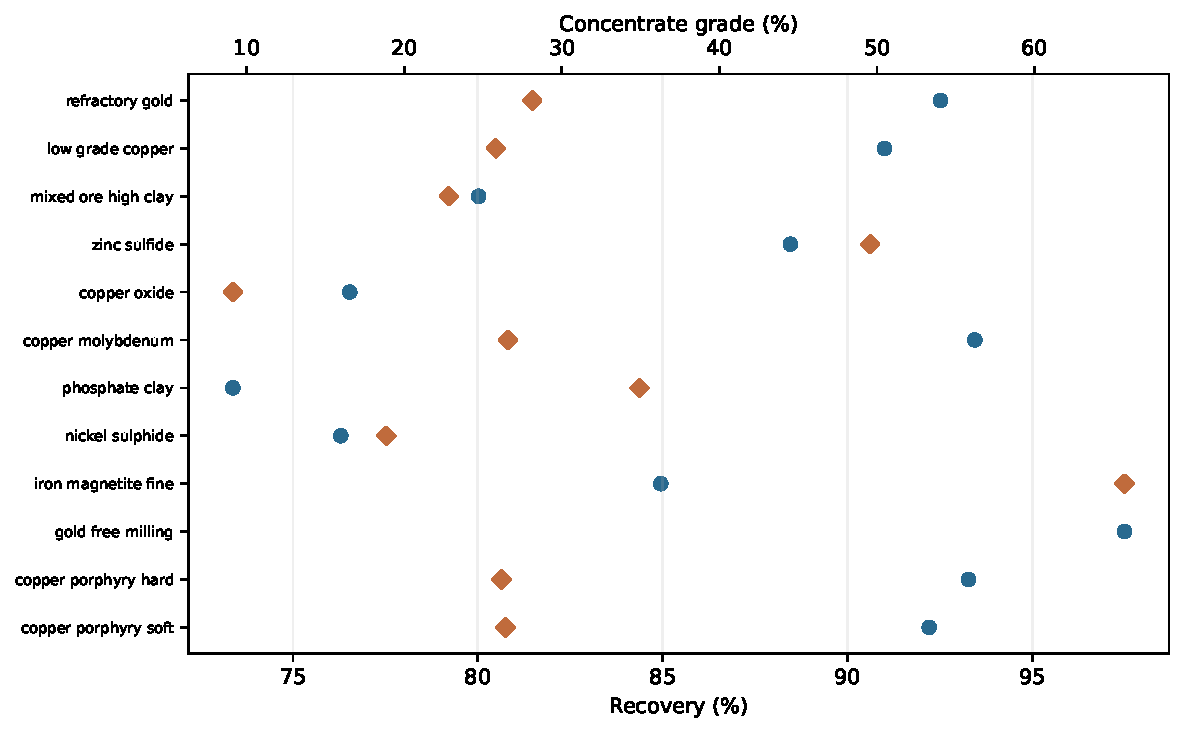
\includegraphics[width=0.94\textwidth]{figures/case-kpis.pdf}
\caption{Modeled recovery and concentrate grade across twelve authored circuits; paired axes preserve their distinct units and the points are not plant measurements.}
\label{fig:case-kpis}
\end{figure}
\begin{figure}[htbp]
\centering
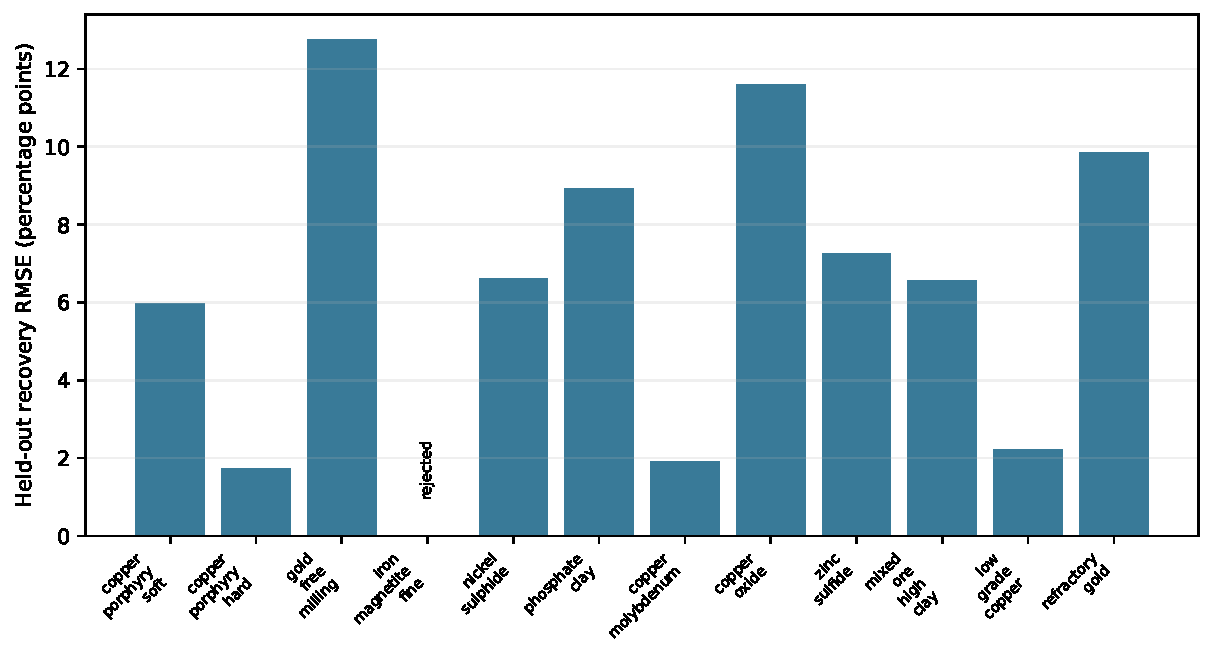
\includegraphics[width=0.94\textwidth]{figures/case-transfer.pdf}
\caption{Neural recovery error for each held-out authored case; the labelled rejection marks a failed range diagnostic and is not assigned a numerical score.}
\label{fig:case-transfer}
\end{figure}
\begin{figure}[htbp]
\centering
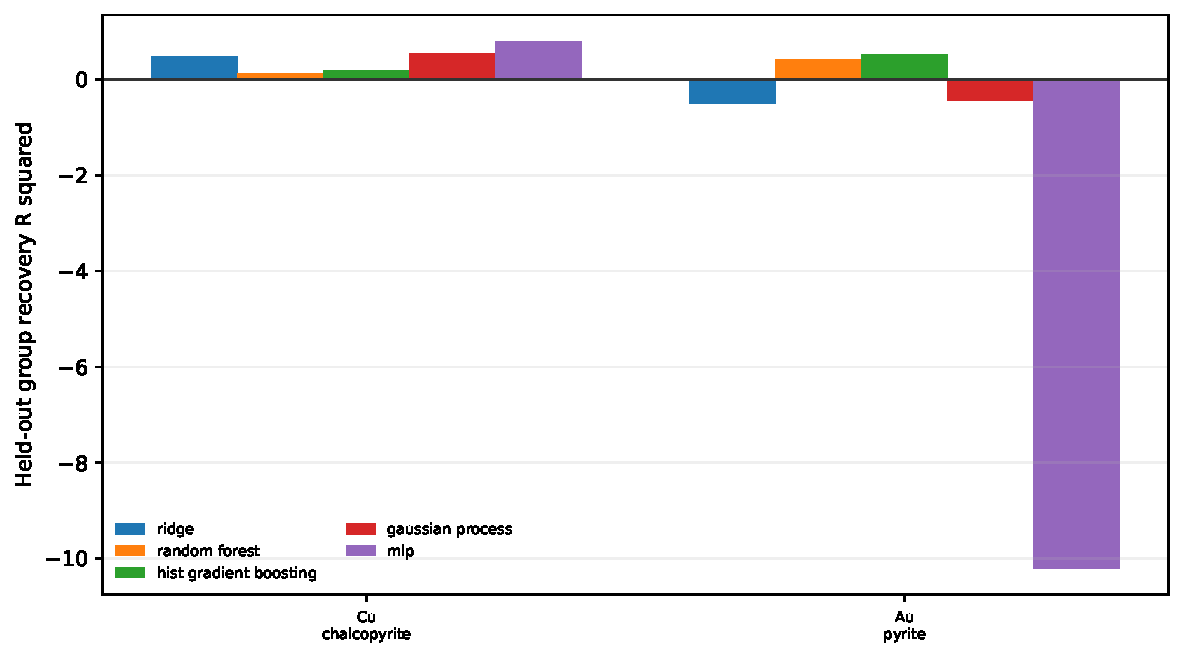
\includegraphics[width=0.94\textwidth]{figures/group-transfer.pdf}
\caption{Recovery determination scores by held-out ore group and model, including negative values that indicate performance below the corresponding cohort-mean predictor.}
\label{fig:group-transfer}
\end{figure}
\begin{figure}[htbp]
\centering
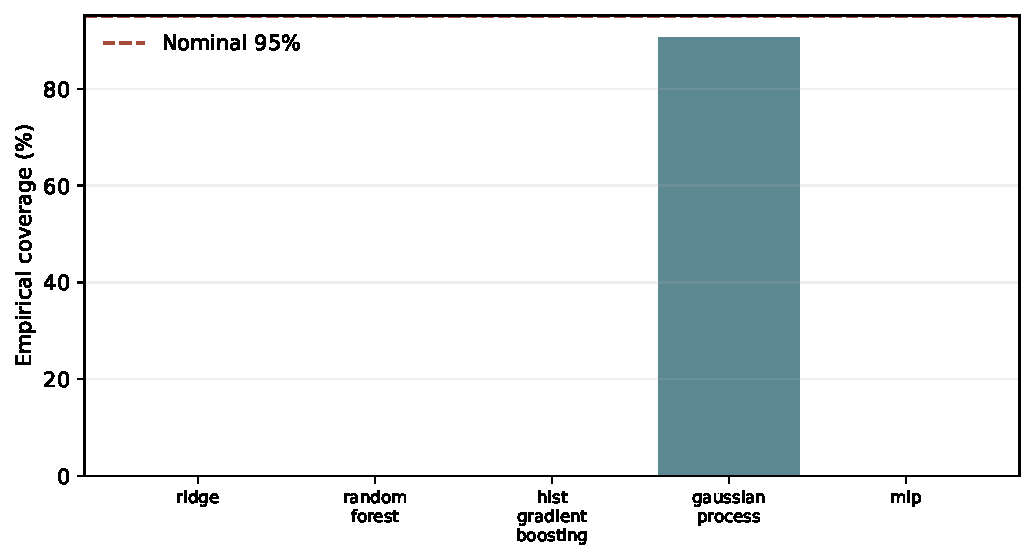
\includegraphics[width=0.94\textwidth]{figures/interval-coverage.pdf}
\caption{Empirical recovery-interval coverage on the interpolation test partition compared with the nominal ninety-five-percent reference level.}
\label{fig:interval-coverage}
\end{figure}
\begin{figure}[htbp]
\centering
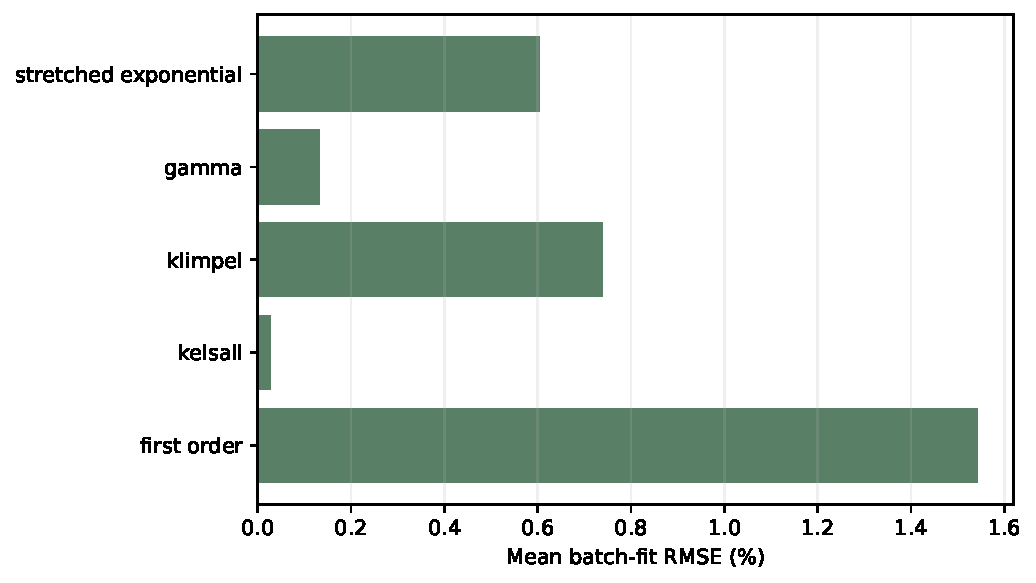
\includegraphics[width=0.94\textwidth]{figures/kinetic-models.pdf}
\caption{Mean fitted batch-recovery error for five implemented kinetic forms over the common virtual batch-record set.}
\label{fig:kinetic-models}
\end{figure}
\begin{figure}[htbp]
\centering
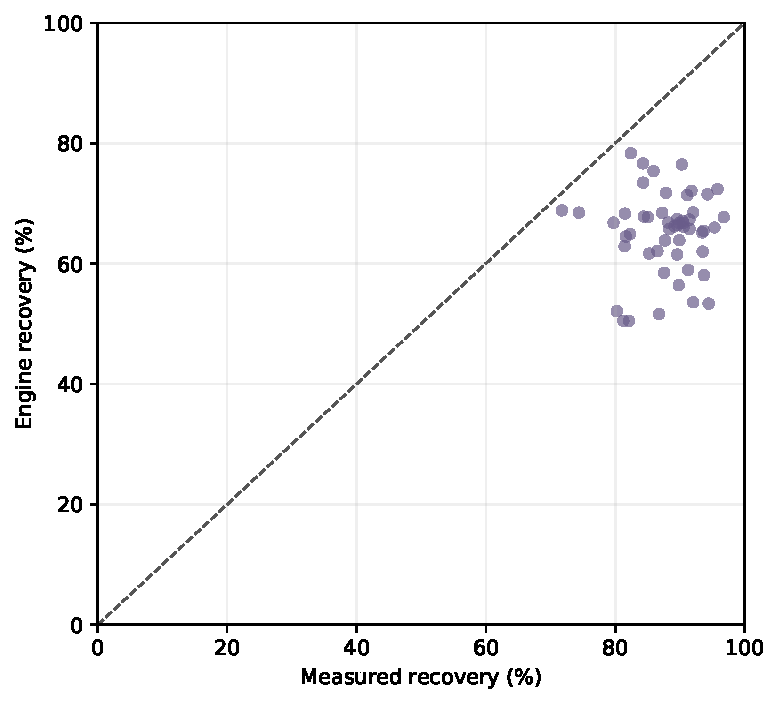
\includegraphics[width=0.94\textwidth]{figures/measured-recovery.pdf}
\caption{Mechanistic engine recovery against 52 external measured samples, with the identity line showing the direction and magnitude of the domain mismatch.}
\label{fig:measured-recovery}
\end{figure}
\begin{figure}[htbp]
\centering
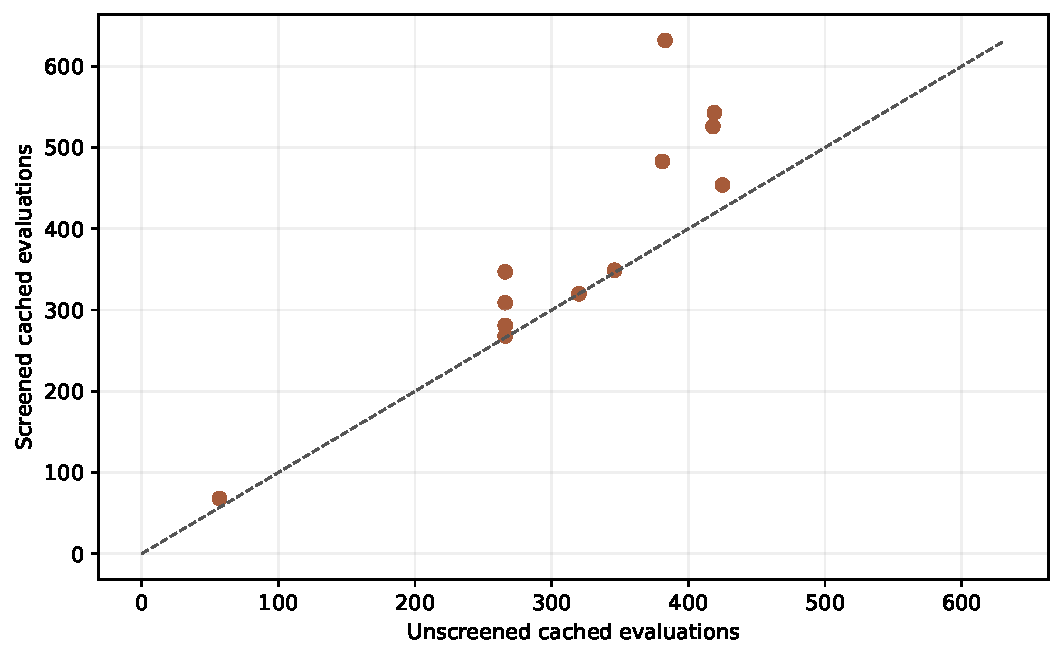
\includegraphics[width=0.94\textwidth]{figures/optimization-cost.pdf}
\caption{Paired cached exact-engine evaluation counts for nominal circuit searches, where points above identity indicate additional calls under surrogate screening.}
\label{fig:optimization-cost}
\end{figure}
\begin{figure}[htbp]
\centering
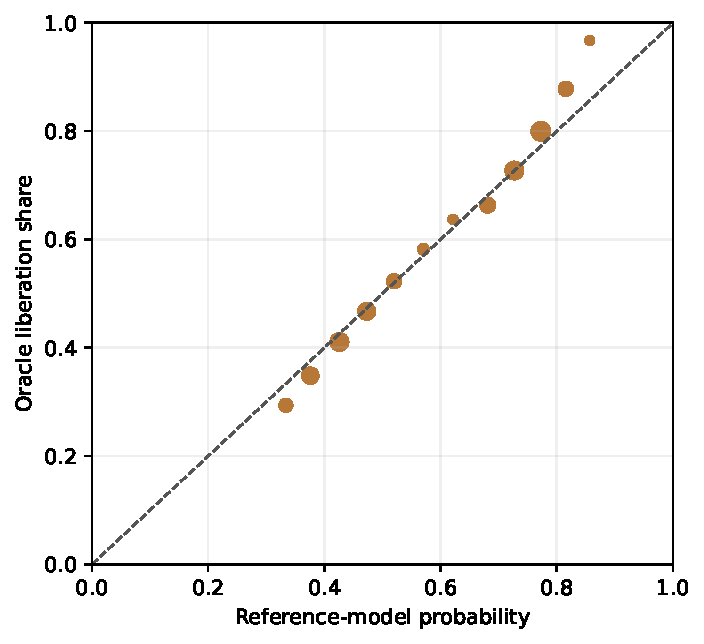
\includegraphics[width=0.94\textwidth]{figures/particle-reference-calibration.pdf}
\caption{Archived particle-reference calibration bins against constructed oracle liberation shares, with marker area proportional to the number of test rows.}
\label{fig:particle-reference-calibration}
\end{figure}
\begin{figure}[htbp]
\centering
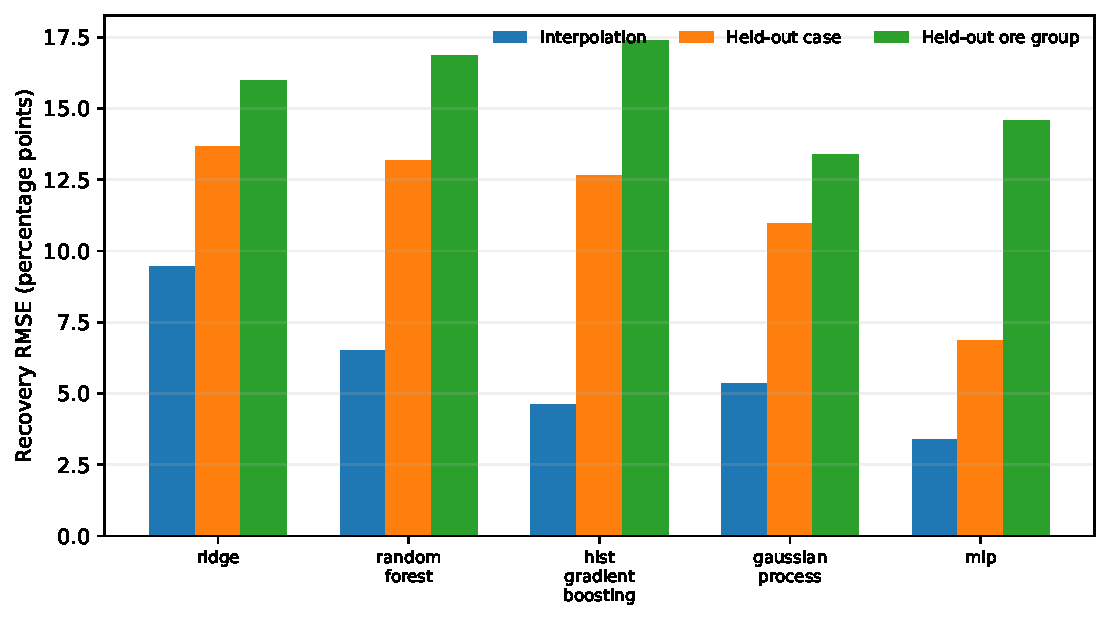
\includegraphics[width=0.94\textwidth]{figures/transfer-protocols.pdf}
\caption{Recovery error for five models under interpolation, whole-case holdout and ore-group holdout, showing that each protocol estimates a different transfer question.}
\label{fig:transfer-protocols}
\end{figure}
\begin{figure}[htbp]
\centering
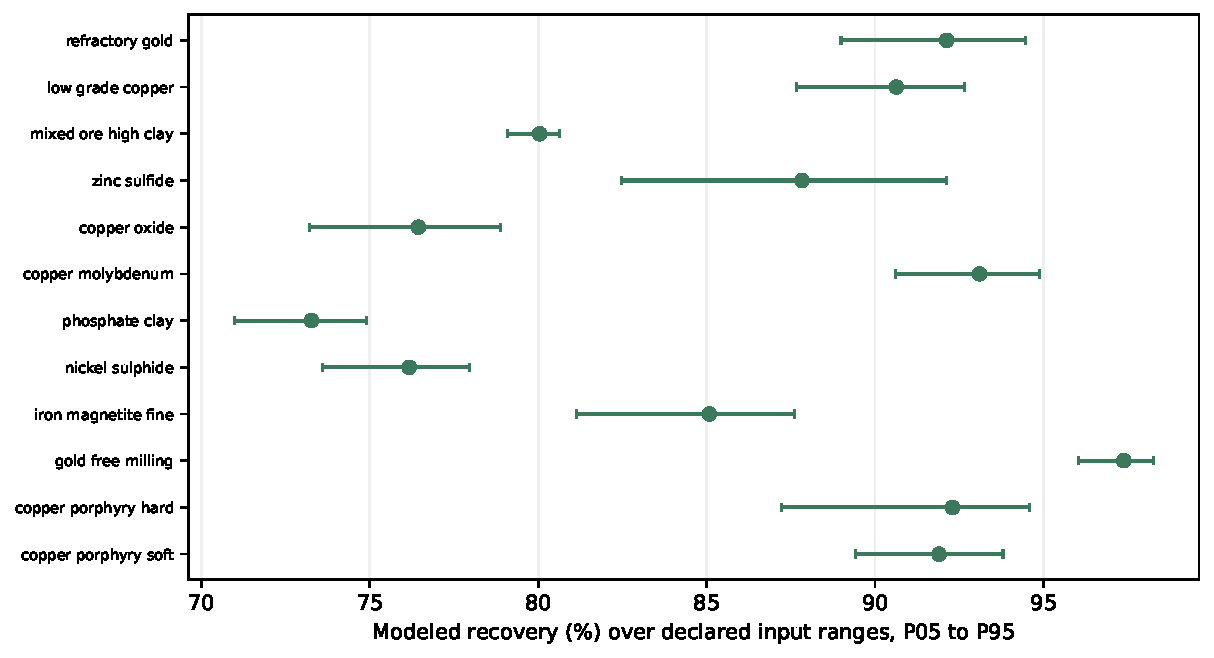
\includegraphics[width=0.94\textwidth]{figures/uncertainty-ranges.pdf}
\caption{Median and fifth-to-ninety-fifth recovery quantiles over each authored case's declared input ranges, not a population-frequency distribution.}
\label{fig:uncertainty-ranges}
\end{figure}
\begin{table}[htbp]
\centering
\small
\caption{Modeled recovery and concentrate grade for twelve authored circuits; the points are simulator outputs, not measured plant observations.}
\label{tab:case-summary}
\begin{tabular}{lrrr}
\toprule
Case & Family & Recovery (\%) & Grade (\%) \\
\midrule
copper\_porphyry\_soft & rougher & 92.21 & 26.42 \\
copper\_porphyry\_hard & rougher & 93.27 & 26.17 \\
gold\_free\_milling & gravity\_rougher & 97.50 & -- \\
iron\_magnetite\_fine & magnetic & 84.95 & 65.72 \\
nickel\_sulphide & deslime\_rougher & 76.30 & 18.86 \\
phosphate\_clay & deslime\_rougher & 73.38 & 34.93 \\
copper\_molybdenum & rougher & 93.45 & 26.58 \\
copper\_oxide & rougher & 76.54 & 9.12 \\
zinc\_sulfide & rougher & 88.46 & 49.58 \\
mixed\_ore\_high\_clay & deslime\_rougher & 80.03 & 22.83 \\
low\_grade\_copper & rougher & 91.01 & 25.82 \\
refractory\_gold & rougher & 92.52 & 28.13 \\
\bottomrule
\end{tabular}
\end{table}
\begin{table}[htbp]
\centering
\small
\caption{Recovery errors by model: interpolation (Interp.), leave-one-case-out (LOCO) and leave-one-ore-group-out (LOGO). Fold columns report scored/rejected.}
\label{tab:learning-summary}
\begin{tabular}{lrrrrr}
\toprule
Model & Interp. & LOCO & LOGO & Case folds & Group folds \\
\midrule
ridge & 9.46 & 13.68 & 15.99 & 12/0 & 7/0 \\
random\_forest & 6.49 & 13.16 & 16.86 & 12/0 & 7/0 \\
hist\_gradient\_boosting & 4.60 & 12.66 & 17.40 & 12/0 & 7/0 \\
gaussian\_process & 5.34 & 10.95 & 13.37 & 12/0 & 7/0 \\
mlp & 3.38 & 6.86 & 14.60 & 11/1 & 6/1 \\
\bottomrule
\end{tabular}
\end{table}
\begin{table}[htbp]
\centering
\small
\caption{Every held-out case result for the multilayer perceptron, preserving gross-range rejections instead of assigning them an artificial error score.}
\label{tab:transfer-folds}
\begin{tabular}{lrrrr}
\toprule
Held-out case & Rows & Status & RMSE (pp) & R squared \\
\midrule
copper\_porphyry\_soft & 256 & scored & 5.98 & 0.854 \\
copper\_porphyry\_hard & 256 & scored & 1.72 & 0.988 \\
gold\_free\_milling & 256 & scored & 12.76 & -1.199 \\
iron\_magnetite\_fine & 256 & rejected-transfer & -- & -- \\
nickel\_sulphide & 256 & scored & 6.61 & 0.472 \\
phosphate\_clay & 256 & scored & 8.93 & 0.437 \\
copper\_molybdenum & 256 & scored & 1.91 & 0.985 \\
copper\_oxide & 256 & scored & 11.60 & 0.185 \\
zinc\_sulfide & 256 & scored & 7.26 & 0.787 \\
mixed\_ore\_high\_clay & 256 & scored & 6.57 & 0.520 \\
low\_grade\_copper & 256 & scored & 2.23 & 0.980 \\
refractory\_gold & 256 & scored & 9.86 & 0.573 \\
\bottomrule
\end{tabular}
\end{table}
\begin{table}[htbp]
\centering
\small
\caption{Model scores for each held-out ore group; negative R squared values remain visible and group identity is not supplied as a predictor.}
\label{tab:group-transfer-evidence}
\begin{tabular}{lrrrrrr}
\toprule
Ore group & Cases & ridge & random\_forest & hist\_gradient\_boosting & gaussian\_process & mlp \\
\midrule
Cu:chalcopyrite & 5 & 0.485 & 0.119 & 0.179 & 0.539 & 0.795 \\
Au:pyrite & 2 & -0.502 & 0.404 & 0.528 & -0.448 & -10.200 \\
\bottomrule
\end{tabular}
\end{table}
\begin{table}[htbp]
\centering
\small
\caption{Five kinetic forms fitted on a common set of virtual batch records; the table reports fit error, circuit-lumping error and convergence.}
\label{tab:kinetics}
\begin{tabular}{lrrrrr}
\toprule
Kinetic form & Fits & RMSE (\%) & Mean lumping error (\%) & Worst error (\%) & Converged \\
\midrule
first\_order & 88 & 1.5422 & 7.559 & 19.132 & 1.000 \\
kelsall & 88 & 0.0280 & 1.806 & 8.473 & 1.000 \\
klimpel & 88 & 0.7397 & 2.805 & 10.555 & 1.000 \\
gamma & 88 & 0.1332 & 1.266 & 5.070 & 1.000 \\
stretched\_exponential & 88 & 0.6051 & 4.763 & 14.732 & 1.000 \\
\bottomrule
\end{tabular}
\end{table}
\begin{table}[htbp]
\centering
\small
\caption{Paired exact-engine evaluation counters at each case's nominal operating point; inference, audits and the later objective-weight path are excluded.}
\label{tab:optimization}
\begin{tabular}{lrrrrr}
\toprule
Case & Unscreened & Screened & Difference & Proposed & Improved \\
\midrule
copper\_porphyry\_soft & 266 & 309 & 43 & 72 & 18 \\
copper\_porphyry\_hard & 418 & 526 & 108 & 186 & 21 \\
gold\_free\_milling & 266 & 268 & 2 & 13 & 5 \\
iron\_magnetite\_fine & 57 & 68 & 11 & 28 & 2 \\
nickel\_sulphide & 346 & 349 & 3 & 32 & 7 \\
phosphate\_clay & 320 & 320 & 0 & 0 & 0 \\
copper\_molybdenum & 266 & 347 & 81 & 108 & 21 \\
copper\_oxide & 383 & 632 & 249 & 154 & 18 \\
zinc\_sulfide & 425 & 454 & 29 & 81 & 16 \\
mixed\_ore\_high\_clay & 419 & 543 & 124 & 146 & 17 \\
low\_grade\_copper & 381 & 483 & 102 & 173 & 22 \\
refractory\_gold & 266 & 281 & 15 & 26 & 9 \\
\bottomrule
\end{tabular}
\end{table}
\begin{table}[htbp]
\centering
\small
\caption{External sample comparison of the mechanistic engine and separate learned data-lane models, with the measured sample count and error units stated.}
\label{tab:measured-data}
\begin{tabular}{lrrr}
\toprule
Method & Samples & Bias (pp) & RMSE (pp) \\
\midrule
Mechanistic engine & 52 & -22.65 & 24.14 \\
train\_mean & 52 & -0.03 & 5.51 \\
ridge & 52 & -0.12 & 5.09 \\
random\_forest & 52 & -0.53 & 5.41 \\
gaussian\_process & 52 & -0.56 & 5.20 \\
\bottomrule
\end{tabular}
\end{table}
\begin{table}[htbp]
\centering
\small
\caption{Seeded recovery quantiles and feasibility probabilities for authored cases, conditional on the declared independent-factor ranges rather than plant-frequency distributions.}
\label{tab:uncertainty}
\begin{tabular}{lrrrr}
\toprule
Case & P05 & P50 & P95 & All constraints \\
\midrule
copper\_porphyry\_soft & 89.41 & 91.90 & 93.80 & 0.820 \\
copper\_porphyry\_hard & 87.23 & 92.30 & 94.58 & 0.539 \\
gold\_free\_milling & 96.04 & 97.38 & 98.25 & 0.820 \\
iron\_magnetite\_fine & 81.13 & 85.08 & 87.61 & 0.523 \\
nickel\_sulphide & 73.59 & 76.17 & 77.96 & 0.789 \\
phosphate\_clay & 70.98 & 73.27 & 74.91 & 0.836 \\
copper\_molybdenum & 90.61 & 93.10 & 94.87 & 0.805 \\
copper\_oxide & 73.21 & 76.44 & 78.88 & 0.875 \\
zinc\_sulfide & 82.46 & 87.83 & 92.13 & 0.438 \\
mixed\_ore\_high\_clay & 79.09 & 80.04 & 80.63 & 0.641 \\
low\_grade\_copper & 87.67 & 90.63 & 92.64 & 0.797 \\
refractory\_gold & 88.99 & 92.12 & 94.46 & 0.789 \\
\bottomrule
\end{tabular}
\end{table}
\begin{table}[htbp]
\centering
\small
\caption{Calibration bins from the archived particle benchmark reference model; marker area is proportional to test rows and the benchmark protocol remains in the source record.}
\label{tab:particle-reference}
\begin{tabular}{lrrr}
\toprule
Case & RMSE & MAE & Bias \\
\midrule
1 & 0.02572 & 0.01994 & -0.00039 \\
2 & 0.01750 & 0.01652 & 0.00043 \\
3 & 0.02070 & 0.01766 & -0.00365 \\
4 & 0.03714 & 0.02721 & 0.00020 \\
\bottomrule
\end{tabular}
\end{table}
